\documentclass[
11pt, % The default document font size, options: 10pt, 11pt, 12pt
codirector, % Uncomment to add a codirector to the title page
]{charter}

% Las tablas se rotulan como ``Tabla'' y no como ``Cuadro'' (predeterminado de babel)
\addto\captionsspanish{\renewcommand{\tablename}{Tabla}}

% El títulos de la memoria, se usa en la carátula y se puede usar el cualquier lugar del documento con el comando \ttitle
\titulo{Optimización de sinopsis de libros mediante predicción de keywords con Machine Learning y SEO} 

% Nombre del posgrado, se usa en la carátula y se puede usar el cualquier lugar del documento con el comando \degreename
%\posgrado{Carrera de Especialización en Sistemas Embebidos} 
%\posgrado{Carrera de Especialización en Internet de las Cosas} 
\posgrado{Carrera de Especialización en Inteligencia Artificial}
%\posgrado{Maestría en Sistemas Embebidos} 
%\posgrado{Maestría en Internet de las cosas}

% Tu nombre, se puede usar el cualquier lugar del documento con el comando \authorname
% IMPORTANTE: no omitir titulaciones ni tildación en los nombres, también se recomienda escribir los nombres completos (tal cual los tienen en su documento)
\autor{Ing. Luis José Paredes Ramirez}

% El nombre del director y co-director, se puede usar el cualquier lugar del documento con el comando \supname y \cosupname y \pertesupname y \pertecosupname
\director{Dr. Ing. Juan Manuel Rodríguez}
\pertenenciaDirector{Universidad de Buenos Aires} 
\codirector{Sebastian Pellizzeri} % para que aparezca en la portada se debe descomentar la opción codirector en los parámetros de documentclass
\pertenenciaCoDirector{Penguin Random House Grupo Editorial}

% Nombre del cliente, quien va a aprobar los resultados del proyecto, se puede usar con el comando \clientename y \empclientename
\cliente{Victoria O\textquotesingle Donnell}
\empresaCliente{Penguin Random House Grupo Editorial}
 
\fechaINICIO{08 de agosto de 2026}		%Fecha de inicio de la cursada de GdP \fechaInicioName
\fechaFINALPlan{13 de octubre de 2026} 	%Fecha de final de cursada de GdP
\fechaFINALTrabajo{15 de mayo de 2027}	%Fecha de defensa pública del trabajo final


\begin{document}

\maketitle
\thispagestyle{empty}
\pagebreak


\thispagestyle{empty}
{\setlength{\parskip}{0pt}
\tableofcontents{}
}
\pagebreak


\section*{Registros de cambios}
\label{sec:registro}


\begin{table}[ht]
\label{tab:registro}
\centering
\begin{tabularx}{\linewidth}{@{}|c|X|c|@{}}
\hline
\rowcolor[HTML]{C0C0C0} 
Revisión & \multicolumn{1}{c|}{\cellcolor[HTML]{C0C0C0}Detalles de los cambios realizados} & Fecha      \\ \hline
0      & Creación del documento                                 &\fechaInicioName \\ \hline
1      & Se completa hasta el punto 5 inclusive                & 07 de septiembre de 2026 \\ \hline
%2      & Se completa hasta el punto 9 inclusive
%		  Se puede agregar algo más \newline
%		  En distintas líneas \newline
%		  Así                                                    & {día} de {mes} de 202X \\ \hline
%3      & Se completa hasta el punto 12 inclusive                & {día} de {mes} de 202X \\ \hline
%4      & Se completa el plan	                                 & {día} de {mes} de 202X \\ \hline

% Si hay más correcciones pasada la versión 4 también se deben especificar acá

\end{tabularx}
\end{table}

\pagebreak



\section*{Acta de constitución del proyecto}
\label{sec:acta}

\begin{flushright}
Buenos Aires, \fechaInicioName
\end{flushright}

\vspace{2cm}

Por medio de la presente se acuerda con el \authorname\hspace{1px} que su Trabajo Final de la \degreename\hspace{1px} se titulará ``\ttitle'' y consistirá en \textcolor{red}{la implementación de un prototipo de un sistema de control de temperatura de una caldera industrial}. El trabajo tendrá un presupuesto preliminar estimado de \textcolor{red}{600} horas y un costo estimado de \textcolor{red}{\$ XXX}, con fecha de inicio el \fechaInicioName\hspace{1px} y fecha de presentación pública el \fechaFinalName.

Se adjunta a esta acta la planificación inicial.

\vfill

% Esta parte se construye sola con la información que hayan cargado en el preámbulo del documento y no debe modificarla
\begin{table}[ht]
\centering
\begin{tabular}{ccc}
\begin{tabular}[c]{@{}c@{}}Dr. Ing. Ariel Lutenberg \\ Director posgrado FIUBA\end{tabular} & \hspace{2cm} & \begin{tabular}[c]{@{}c@{}}\clientename \\ \empclientename \end{tabular} \vspace{2.5cm} \\ 
\multicolumn{3}{c}{\begin{tabular}[c]{@{}c@{}} \supname \\ Director del Trabajo Final\end{tabular}} \vspace{2.5cm} \\
\end{tabular}
\end{table}




\section{1. Descripción técnica-conceptual del proyecto a realizar}
\label{sec:descripcion}

El proyecto se desarrolla como una iniciativa interna de Penguin Random House Grupo Editorial Argentina, empresa que edita, publica y distribuye libros en formato papel, digital y audio para lectores de todas las edades. El responsable se desempeña en esa organización como \textit{Machine Learning Engineer}, condición que habilita el acceso al catálogo editorial, a los datos internos de posicionamiento y a una cuenta paga de la interfaz de programación de aplicaciones (API) de DataForSEO.

En una tienda en línea, la sinopsis es el principal texto indexable de la ficha de cada libro y determina en buena medida que un lector potencial encuentre el título al buscar por género, autor o temática. Sin embargo, ese texto se redacta con criterio editorial y no contempla la demanda real de búsqueda. La selección manual de \textit{keywords}, o palabras clave, exige tiempo de especialistas y no escala a un catálogo de miles de títulos, por lo que en la práctica solo alcanza a las novedades y a los libros más vendidos.

La optimización para motores de búsqueda (SEO, por su sigla en inglés) reúne las técnicas que mejoran la posición de un sitio en los resultados de los buscadores, principalmente Google. El tráfico se concentra en los primeros lugares de la página de resultados del buscador (SERP, por su sigla en inglés), de modo que elegir las \textit{keywords} adecuadas para cada contenido es una decisión de alto impacto comercial.

Las suites comerciales de SEO informan el volumen de búsqueda y la dificultad estimada de cada \textit{keyword}, pero esas métricas son agregadas y no anticipan cómo posiciona un dominio determinado frente a su competencia directa. Los modelos grandes de lenguaje (LLM, por su sigla en inglés), por su parte, generan con facilidad textos orientados al posicionamiento, aunque sin anclaje en datos propios y sin garantía de fidelidad al contenido del libro. Entre ambas carencias, la decisión final queda librada a la intuición del redactor.

La solución propuesta consta de dos etapas. En la primera, un modelo de aprendizaje automático (ML, por su sigla en inglés) estima, para cada par formado por un libro y una \textit{keyword}, la probabilidad de que el dominio de la editorial posicione mejor que el de su competencia, y ordena las palabras clave según ese criterio. En la segunda, un generador basado en un LLM reescribe la sinopsis original e incorpora las \textit{keywords} priorizadas, bajo restricciones de extensión, tono y fidelidad al argumento del libro.

La propuesta de valor reside en reemplazar una tarea artesanal por un procedimiento sistemático y reproducible, aplicable a cualquier libro del catálogo. La innovación pasa por dos aspectos: el modelo se entrena con la señal de competencia observada en la SERP entre dos catálogos que disputan las mismas audiencias, y la generación queda condicionada por esa señal y verificada de forma automática antes de la revisión editorial. Como caso de estudio se utilizan los catálogos de Penguin Random House Argentina y de Planeta, que compiten en géneros equivalentes, como la novela romántica, la fantasía juvenil, la no ficción y la autoayuda.

En la figura \ref{fig:diagBloques} se presenta el diagrama en bloques del sistema. Se observa que el flujo parte de tres fuentes de datos: la API de DataForSEO, los datos internos de la editorial y el catálogo de la competencia obtenido mediante \textit{scraping}. El bloque de ingesta consolida esa información en un conjunto de datos único que vincula libro, \textit{keyword}, dirección web y posición histórica. Sobre ese conjunto se construyen las variables que alimentan al modelo de predicción, cuya salida es la lista de palabras clave priorizadas para cada título.

\begin{figure}[htpb]
\centering
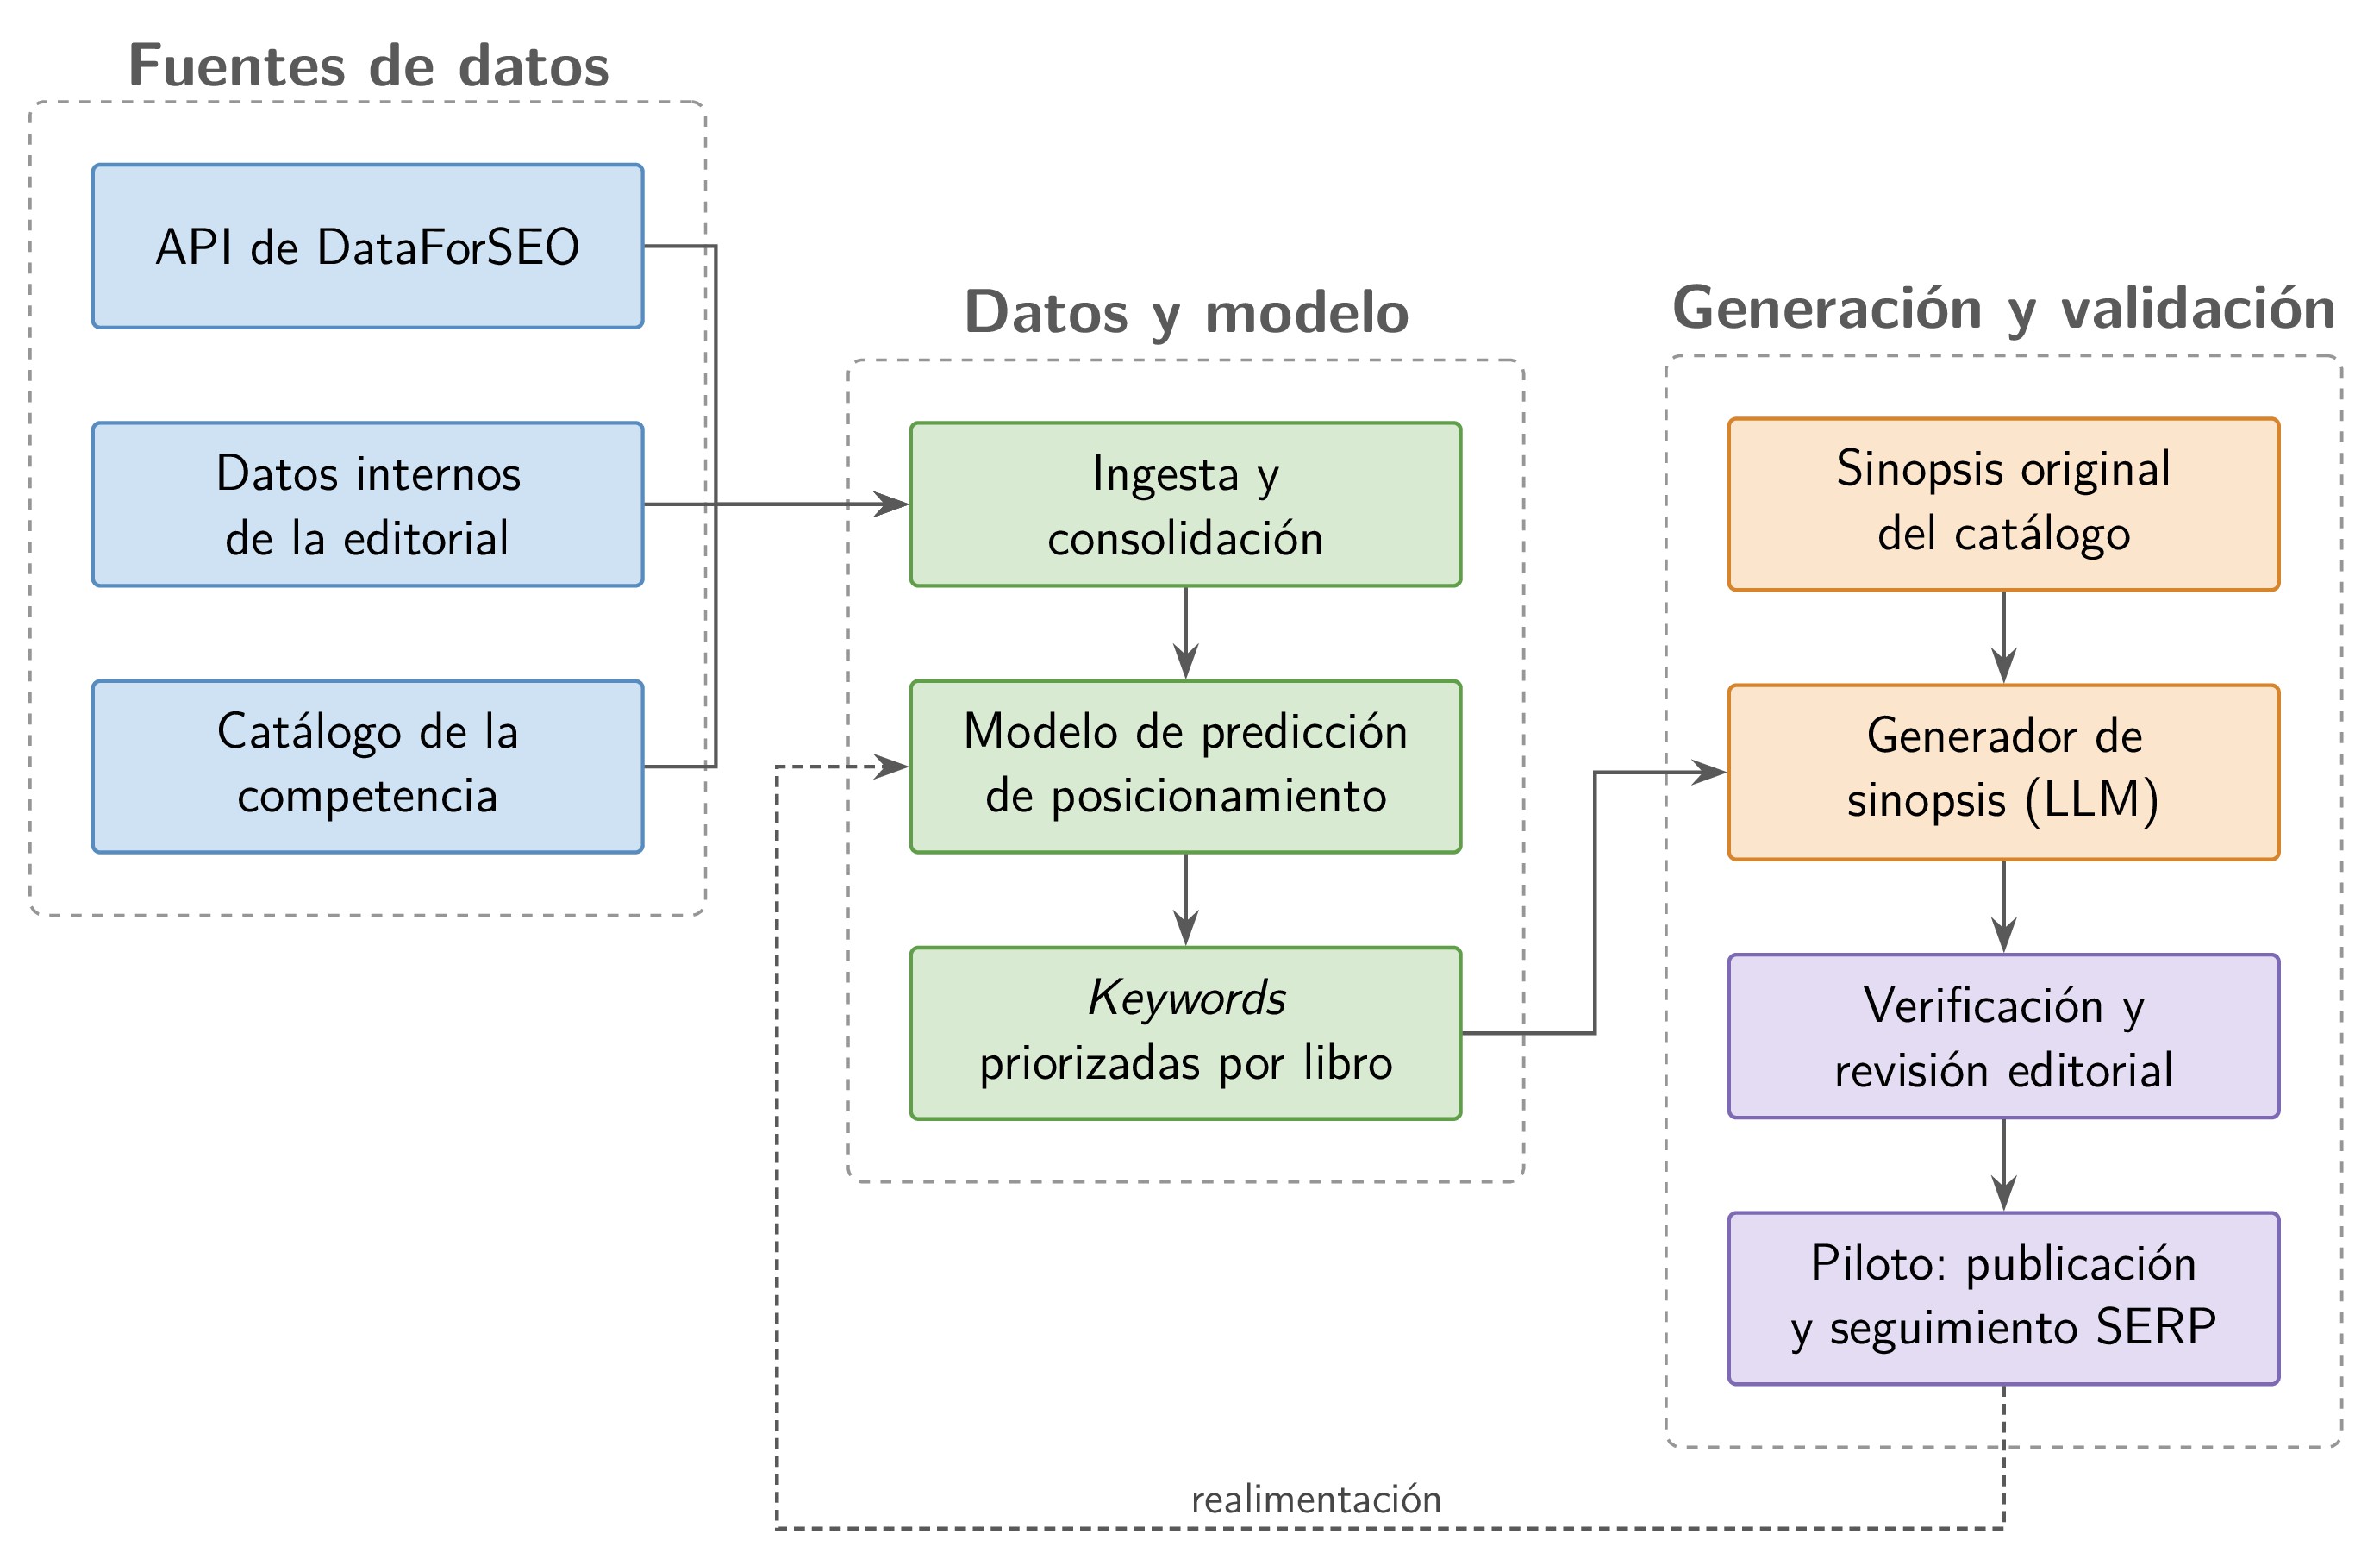
\includegraphics[width=\textwidth]{./Figuras/diagBloques.png}
\caption{Diagrama en bloques del sistema.}
\label{fig:diagBloques}
\end{figure}

El generador de sinopsis recibe el texto original y esas palabras clave, y produce una versión candidata. Un módulo de verificación automática controla la similitud semántica con el texto original, la extensión y la presencia efectiva de las \textit{keywords}; solo las candidatas que superan esos controles pasan a revisión editorial. Las sinopsis aprobadas se publican en un piloto acotado, cuyo seguimiento de posiciones en la SERP realimenta el conjunto de datos y habilita un nuevo entrenamiento del modelo.
 
\section{2. Identificación y análisis de los interesados}
\label{sec:interesados}

El proyecto se desarrolla internamente por el equipo de Analítica Avanzada de Penguin Random House Grupo Editorial. En la tabla \ref{tag:interesados} se identifican los interesados del proyecto y el rol que ocupa cada uno.

\begin{table}[ht]
\caption{Identificación de los interesados.}
\label{tag:interesados}
\begin{tabularx}{\linewidth}{@{}|l|X|X|l|@{}}
\hline
\rowcolor[HTML]{C0C0C0}
Rol           & Nombre y Apellido & Organización 	& Puesto 	\\ \hline
Auspiciante   & -   & \empclientename &			\\ \hline
Cliente       & \clientename      &\empclientename	& Cientifica de Datos \\ \hline
Responsable   & \authorname       & \empclientename & Machine Learning Engineer 	\\ \hline
Orientador    & \supname	      & \pertesupname 	& Director del Trabajo Final \\ \hline
Orientador    & \cosupname	      & \pertecosupname & Codirector del Trabajo Final \\ \hline
\end{tabularx}
%\caption{Identificación de los interesados.}
\end{table}


\begin{itemize}
	\item Auspiciante: la editorial aporta las horas de trabajo del responsable, el acceso a los datos internos y el crédito de la API de DataForSEO. Cualquier consumo por encima de lo previsto requiere una autorización expresa, de modo que conviene acotar las consultas al proveedor desde el diseño del conjunto de datos.
	\item Cliente: valida los entregables y define qué títulos integran el piloto. Su disponibilidad es acotada, por lo que las instancias de validación deben planificarse con anticipación y concentrarse en pocas reuniones.
	\item Orientadores: el director aporta el encuadre metodológico y la supervisión académica del Trabajo Final; el codirector, el conocimiento del negocio editorial y de los sistemas internos. Este último también fija prioridades dentro de la empresa.
\end{itemize}


\section{3. Propósito del proyecto}
\label{sec:proposito}

Aumentar la visibilidad orgánica del catálogo de la editorial en los resultados de búsqueda mediante sinopsis optimizadas con palabras clave seleccionadas por un modelo de aprendizaje automático. Se busca reemplazar la curaduría manual de \textit{keywords}, hoy limitada a un puñado de títulos, por un procedimiento sistemático, reproducible y aplicable a la escala del catálogo completo, que priorice las palabras clave con mayor probabilidad de posicionamiento y produzca sinopsis fieles al contenido original.

\section{4. Alcance del proyecto}
\label{sec:alcance}

El proyecto incluye:

\begin{itemize}
	\item La construcción del conjunto de datos de posicionamiento.
		\begin{itemize}
		\item Extracción de datos de SEO de ambos dominios mediante la API de DataForSEO.
		\item Incorporación de los datos internos de la editorial: catálogo, series históricas de Google Trends y resultados de proyectos de SEO previos.
		\item Obtención del catálogo de la competencia mediante \textit{scraping} de su sitio web.
		\item Consolidación, limpieza y versionado del conjunto de datos.
		\end{itemize}
	\item El análisis exploratorio de los datos y la construcción de las variables predictoras.
	\item El desarrollo del modelo de predicción de posicionamiento.
		\begin{itemize}
		\item Entrenamiento y comparación de al menos dos algoritmos alternativos.
		\item Definición de la métrica de priorización de \textit{keywords} por libro.
		\item Validación contra las posiciones históricas observadas.
		\end{itemize}
	\item El desarrollo del generador de sinopsis basado en un LLM comercial, con sus restricciones de extensión, tono y uso de palabras clave.
	\item El módulo de verificación automática de las sinopsis candidatas: fidelidad semántica respecto del texto original, extensión y presencia efectiva de las \textit{keywords}.
	\item La ejecución de un piloto acotado sobre un subconjunto del catálogo, con publicación de las sinopsis aprobadas y seguimiento de las posiciones en la SERP durante la ventana de medición acordada.
	\item La documentación del sistema, el código fuente y la memoria del Trabajo Final.
\end{itemize}

El presente proyecto no incluye:

\begin{itemize}
	\item La integración productiva con el gestor de contenidos de la tienda en línea: la carga de las sinopsis del piloto se realiza por los canales que la editorial ya utiliza.
	\item El despliegue sobre la totalidad del catálogo ni la puesta en producción del sistema.
	\item La medición del impacto en ventas o en ingresos, que excede la ventana temporal del proyecto.
	\item La optimización de otros factores de SEO, tales como el enlazado interno, el rendimiento del sitio o los metadatos distintos de la sinopsis.
	\item El entrenamiento de un modelo de lenguaje propio.
	\item La traducción o adaptación de sinopsis a otros mercados de habla hispana.
	\item El soporte y el mantenimiento posteriores al cierre del proyecto.
\end{itemize}


\section{5. Supuestos del proyecto}
\label{sec:supuestos}

Para el desarrollo del presente proyecto se supone que:

\begin{itemize}
	\item La editorial mantiene la autorización para utilizar el catálogo, las sinopsis y los datos internos de posicionamiento con fines académicos, y admite la publicación de resultados agregados en la memoria del Trabajo Final.
	\item El acceso a la API de DataForSEO continúa vigente durante toda la ejecución y el crédito contratado alcanza para el volumen de consultas previsto.
	\item Se dispone de acceso a una API de LLM comercial, con un costo por consulta compatible con el presupuesto asignado.
	\item El sitio web de la competencia permite obtener su catálogo mediante \textit{scraping}. Si esa vía no resulta viable, el análisis se limita al catálogo interno de la editorial.
	\item El área de marketing digital habilita la publicación de las sinopsis del piloto dentro de los plazos planificados.
	\item El algoritmo de Google no sufre cambios de magnitud durante la ventana de medición del piloto, de modo que las variaciones observadas resultan atribuibles a las sinopsis modificadas.
	\item Los datos históricos de posicionamiento cubren un período suficiente para entrenar y validar el modelo.
	\item El responsable dispone de una carga horaria semanal sostenida y compatible con el cronograma, y cuenta con el equipamiento y los servicios de cómputo necesarios.
	\item Las condiciones macroeconómicas no alteran de forma significativa el costo en pesos de los servicios contratados en moneda extranjera.
\end{itemize}

\section{6. Requerimientos}
\label{sec:requerimientos}

\begin{consigna}{red} % ELIMINAR \begin{consigna}{red} y \end{consigna}{red} en las secciones que vayan completando para cada entrega parcial.
Los requerimientos deben enumerarse y de ser posible estar agrupados por afinidad, por ejemplo:

\begin{enumerate}
	\item Requerimientos funcionales:
		\begin{enumerate}
			\item El sistema debe...
			\item Tal componente debe...
			\item El usuario debe poder...
		\end{enumerate}
	\item Requerimientos de documentación:
		\begin{enumerate}
			\item Requerimiento 1.
			\item Requerimiento 2 (prioridad menor)
		\end{enumerate}
	\item Requerimiento de testing...
	\item Requerimientos de la interfaz...
	\item Requerimientos interoperabilidad...
	\item etc...
\end{enumerate}

Leyendo los requerimientos se debe poder interpretar cómo será el proyecto y su funcionalidad.

Indicar claramente cuál es la prioridad entre los distintos requerimientos y si hay requerimientos opcionales. 

\textbf{¡¡¡No olvidarse de que los requerimientos incluyen a las regulaciones y normas vigentes!!!}

Y al escribirlos seguir las siguientes reglas:
\begin{itemize}
	\item Ser breve y conciso (nadie lee cosas largas). 
	\item Ser específico: no dejar lugar a confusiones.
	\item Expresar los requerimientos en términos que sean cuantificables y medibles.
\end{itemize}

\end{consigna} % ELIMINAR \begin{consigna}{red} y \end{consigna}{red} en las secciones que vayan completando para cada entrega parcial.

\section{7. Historias de usuarios (\textit{Product backlog})}
\label{sec:backlog}

\begin{consigna}{red}
Descripción: en esta sección se deben incluir las historias de usuarios y su ponderación (\textit{history points}). Recordar que las historias de usuarios son descripciones cortas y simples de una característica contada desde la perspectiva de la persona que desea la nueva capacidad, generalmente un usuario o cliente del sistema. La ponderación es un número entero que representa el tamaño de la historia comparada con otras historias de similar tipo.

Se debe indicar explícitamente el criterio para calcular los \textit{story points} de cada historia.

El formato propuesto es: 
\begin{enumerate}
\item ``Como [rol] quiero [tal cosa] para [tal otra cosa]."

\textit{Story points}: 8 (complejidad: 3, dificultad: 2, incertidumbre: 3)
\end{enumerate}
\end{consigna}

\section{8. Entregables principales del proyecto}
\label{sec:entregables}

\begin{consigna}{red}
Los entregables del proyecto son (ejemplo):

\begin{itemize}
	\item Manual de usuario.
	\item Diagrama de circuitos esquemáticos.
	\item Código fuente del firmware.
	\item Diagrama de instalación.
	\item Memoria del trabajo final.
	\item etc...
\end{itemize}
\end{consigna}

\section{9. Desglose del trabajo en tareas}
\label{sec:wbs}

\begin{consigna}{red}
El WBS debe tener relación directa o indirecta con los requerimientos.  Son todas las actividades que se harán en el proyecto para dar cumplimiento a los requerimientos. Se recomienda mostrar el WBS mediante una lista indexada:

\begin{enumerate}
\item Grupo de tareas 1 (suma h)
	\begin{enumerate}
	\item Tarea 1 (tantas h)
	\item Tarea 2 (tantas h)
	\item Tarea 3 (tantas h)
	\end{enumerate}
\item Grupo de tareas 2 (suma h)
	\begin{enumerate}
	\item Tarea 1 (tantas h)
	\item Tarea 2 (tantas h)
	\item Tarea 3 (tantas h)
	\end{enumerate}
\item Grupo de tareas 3 (suma h)
	\begin{enumerate}
	\item Tarea 1 (tantas h)
	\item Tarea 2 (tantas h)
	\item Tarea 3 (tantas h)
	\item Tarea 4 (tantas h)
	\item Tarea 5 (tantas h)
	\end{enumerate}
\end{enumerate}

Cantidad total de horas: tantas.

\textbf{¡Importante!:} la unidad de horas es h y va separada por espacio del número. Es incorrecto escribir ``23hs".

\textbf{Se recomienda que no haya ninguna tarea que lleve más de 40 h.} De ser así se recomienda dividirla en tareas de menor duración.

\end{consigna}

\section{10. Diagrama de Activity On Node}
\label{sec:AoN}

\begin{consigna}{red}
Armar el AoN a partir del WBS definido en la etapa anterior.

Una herramienta simple para desarrollar los diagramas es el Draw.io (\url{https://app.diagrams.net/}).
\href{https://app.diagrams.net}{Draw.io}


\begin{figure}[htpb]
\centering 
\includegraphics[width=.8\textwidth]{./Figuras/AoN.png}
\caption{Diagrama de \textit{Activity on Node}.}
\label{fig:AoN}
\end{figure}

Indicar claramente en qué unidades están expresados los tiempos.
De ser necesario indicar los caminos semi críticos y analizar sus tiempos mediante un cuadro.
Es recomendable usar colores y un cuadro indicativo describiendo qué representa cada color.

\end{consigna}

\section{11. Diagrama de Gantt}
\label{sec:gantt}

\begin{consigna}{red}
Existen muchos programas y recursos \textit{online} para hacer diagramas de Gantt, entre los cuales destacamos:

\begin{itemize}
\item Planner
\item GanttProject
\item Trello + \textit{plugins}. En el siguiente link hay un tutorial oficial: \\ \url{https://blog.trello.com/es/diagrama-de-gantt-de-un-proyecto}
\item Creately, herramienta online colaborativa. \\\url{https://creately.com/diagram/example/ieb3p3ml/LaTeX}
\item Se puede hacer en latex con el paquete \textit{pgfgantt}\\ \url{http://ctan.dcc.uchile.cl/graphics/pgf/contrib/pgfgantt/pgfgantt.pdf}
\end{itemize}

Pegar acá una captura de pantalla del diagrama de Gantt, cuidando que la letra sea suficientemente grande como para ser legible. 
Si el diagrama queda demasiado ancho, se puede pegar primero la ``tabla'' del Gantt y luego pegar la parte del diagrama de barras del diagrama de Gantt.

Configurar el software para que en la parte de la tabla muestre los códigos del EDT (WBS).\\
Configurar el software para que al lado de cada barra muestre el nombre de cada tarea.\\
Revisar que la fecha de finalización coincida con lo indicado en el Acta Constitutiva.

En la figura \ref{fig:gantt}, se muestra un ejemplo de diagrama de gantt realizado con el paquete de \textit{pgfgantt}. 
En la plantilla pueden ver el código que lo genera y usarlo de base para construir el propio.

Las fechas pueden ser calculadas utilizando alguna de las herramientas antes citadas. Sin embargo, el siguiente ejemplo
fue elaborado utilizando 
\href{https://docs.google.com/spreadsheets/d/1fBz8NhSpc4tkkhz3KjJCbh1nR_ltDkfEcZi4tZXduqs}{esta hoja de cálculo}.

Es importante destacar que el ancho del diagrama estará dado por la longitud del texto utilizado para las tareas 
(Ejemplo: tarea 1, tarea 2, etcétera) y el valor \textit{x unit}. Para mejorar la apariencia del diagrama, es necesario
ajustar este valor y, quizás, acortar los nombres de las tareas.

\begin{figure}[htpb]
  \begin{center}
    \begin{ganttchart}[
      time slot unit=day,
      time slot format=isodate,
      x unit=0.038cm,
      y unit title=0.7cm,
      y unit chart=0.6cm,
      milestone/.append style={xscale=4}
      ]{2021-03-05}{2021-12-16}
      \gantttitlecalendar*{2021-03-05}{2021-12-16}{year} \\
      \gantttitlecalendar*{2021-03-05}{2021-12-16}{month} \\
      \ganttgroup{Duración Total}{2021-03-05}{2021-12-16} \\
      %%%%%%%%%%%%%%%%%Organización
      \ganttgroup{Organización}{2021-03-05}{2021-04-16} \\
      \ganttbar{Planificación del proyecto}{2021-03-05}{2021-04-15} \\
      %%%%%%%%%%%%%%%%%Ejecución
      \ganttgroup{Ejecución}{2021-04-16}{2021-10-21} \\
      \ganttbar{Tarea 1}{2021-04-16}{2021-04-29} \\
      \ganttbar{Tarea 2}{2021-04-30}{2021-05-13} \\
      \ganttbar{Tarea 3}{2021-05-14}{2021-05-27} \\
      \ganttbar{Tarea 4}{2021-05-28}{2021-07-12} \\
      \ganttbar{Tarea 5}{2021-07-13}{2021-08-09} \\
      \ganttbar{Tarea 6}{2021-08-10}{2021-09-23} \\
      \ganttbar{Tarea 7}{2021-09-24}{2021-09-30} \\
      \ganttbar{Tarea 8}{2021-10-01}{2021-10-14} \\
      \ganttbar{Tarea 9}{2021-10-15}{2021-10-21} \\
      % %%%%%%%%%%%%%%%%%Finalización
      \ganttgroup{Finalización}{2021-10-22}{2021-12-16} \\
      \ganttbar{Memoria v1}{2021-10-22}{2021-11-04} \\
      \ganttbar{Memoria v2}{2021-11-05}{2021-11-18} \\
      \ganttbar{Memoria final}{2021-11-19}{2021-12-02} \\
      % La fecha del siguiente milestone es la fecha en que terminamos la memoria
      \ganttmilestone{Enviar memoria al director}{2021-12-02} \\
      \ganttbar{Elaborar la presentación}{2021-12-03}{2021-12-16} \\
      \ganttmilestone{Ensayo de la presentación}{2021-12-16} \\
      %%%%%%%%%%%%%%%%%%%%%%%%%%%%%%%%%%%%%%%%%%%%%%%%%%%%%%%%%%%%%%%
    \end{ganttchart}
  \end{center}
  \caption{Diagrama de gantt de ejemplo}
  \label{fig:gantt}
\end{figure}


\begin{landscape}
\begin{figure}[htpb]
\centering 
\includegraphics[height=.85\textheight]{./Figuras/Gantt-2.png}
\caption{Ejemplo de diagrama de Gantt (apaisado).} %Modificar este título acorde.
\label{fig:diagGantt}
\end{figure}

\end{landscape}

\end{consigna}


\section{12. Presupuesto detallado del proyecto}
\label{sec:presupuesto}

\begin{consigna}{red}
Si el proyecto es complejo entonces separarlo en partes:
\begin{itemize}
	\item Un total global, indicando el subtotal acumulado por cada una de las áreas.
	\item El desglose detallado del subtotal de cada una de las áreas.
\end{itemize}

IMPORTANTE: No olvidarse de considerar los COSTOS INDIRECTOS.

Incluir la aclaración de si se emplea como moneda el peso argentino (ARS) o si se usa moneda extranjera (USD, EUR, etc). Si es en moneda extranjera se debe indicar la tasa de conversión respecto a la moneda local en una fecha dada.

\end{consigna}

\begin{table}[htpb]
\centering
\begin{tabularx}{\linewidth}{@{}|X|c|r|r|@{}}
\hline
\rowcolor[HTML]{C0C0C0} 
\multicolumn{4}{|c|}{\cellcolor[HTML]{C0C0C0}COSTOS DIRECTOS} \\ \hline
\rowcolor[HTML]{C0C0C0} 
Descripción &
  \multicolumn{1}{c|}{\cellcolor[HTML]{C0C0C0}Cantidad} &
  \multicolumn{1}{c|}{\cellcolor[HTML]{C0C0C0}Valor unitario} &
  \multicolumn{1}{c|}{\cellcolor[HTML]{C0C0C0}Valor total} \\ \hline
 &
  \multicolumn{1}{c|}{} &
  \multicolumn{1}{c|}{} &
  \multicolumn{1}{c|}{} \\ \hline
 &
  \multicolumn{1}{c|}{} &
  \multicolumn{1}{c|}{} &
  \multicolumn{1}{c|}{} \\ \hline
\multicolumn{1}{|l|}{} &
   &
   &
   \\ \hline
\multicolumn{1}{|l|}{} &
   &
   &
   \\ \hline
\multicolumn{3}{|c|}{SUBTOTAL} &
  \multicolumn{1}{c|}{} \\ \hline
\rowcolor[HTML]{C0C0C0} 
\multicolumn{4}{|c|}{\cellcolor[HTML]{C0C0C0}COSTOS INDIRECTOS} \\ \hline
\rowcolor[HTML]{C0C0C0} 
Descripción &
  \multicolumn{1}{c|}{\cellcolor[HTML]{C0C0C0}Cantidad} &
  \multicolumn{1}{c|}{\cellcolor[HTML]{C0C0C0}Valor unitario} &
  \multicolumn{1}{c|}{\cellcolor[HTML]{C0C0C0}Valor total} \\ \hline
\multicolumn{1}{|l|}{} &
   &
   &
   \\ \hline
\multicolumn{1}{|l|}{} &
   &
   &
   \\ \hline
\multicolumn{1}{|l|}{} &
   &
   &
   \\ \hline
\multicolumn{3}{|c|}{SUBTOTAL} &
  \multicolumn{1}{c|}{} \\ \hline
\rowcolor[HTML]{C0C0C0}
\multicolumn{3}{|c|}{TOTAL} &
   \\ \hline
\end{tabularx}%
\end{table}


\section{13. Gestión de riesgos}
\label{sec:riesgos}

\begin{consigna}{red}
a) Identificación de los riesgos (al menos cinco) y estimación de sus consecuencias:
 
Riesgo 1: detallar el riesgo (riesgo es algo que si ocurre altera los planes previstos de forma negativa)
\begin{itemize}
	\item Severidad (S): mientras más severo, más alto es el número (usar números del 1 al 10).\\
	Justificar el motivo por el cual se asigna determinado número de severidad (S).
	\item Probabilidad de ocurrencia (O): mientras más probable, más alto es el número (usar del 1 al 10).\\
	Justificar el motivo por el cual se asigna determinado número de (O). 
\end{itemize}   

Riesgo 2:
\begin{itemize}
	\item Severidad (S): X.\\
	Justificación...
	\item Ocurrencia (O): Y.\\
	Justificación...
\end{itemize}

Riesgo 3:
\begin{itemize}
	\item Severidad (S):  X.\\
	Justificación...
	\item Ocurrencia (O): Y.\\
	Justificación...
\end{itemize}


b) Tabla de gestión de riesgos:      (El RPN se calcula como RPN=SxO)

\begin{table}[htpb]
\centering
\begin{tabularx}{\linewidth}{@{}|X|c|c|c|c|c|c|@{}}
\hline
\rowcolor[HTML]{C0C0C0} 
Riesgo & S & O & RPN & S* & O* & RPN* \\ \hline
       &   &   &     &    &    &      \\ \hline
       &   &   &     &    &    &      \\ \hline
       &   &   &     &    &    &      \\ \hline
       &   &   &     &    &    &      \\ \hline
       &   &   &     &    &    &      \\ \hline
\end{tabularx}%
\end{table}

Criterio adoptado: 

Se tomarán medidas de mitigación en los riesgos cuyos números de RPN sean mayores a...

Nota: los valores marcados con (*) en la tabla corresponden luego de haber aplicado la mitigación.

c) Plan de mitigación de los riesgos que originalmente excedían el RPN máximo establecido:
 
Riesgo 1: plan de mitigación (si por el RPN fuera necesario elaborar un plan de mitigación).
  Nueva asignación de S y O, con su respectiva justificación:
  \begin{itemize}
	\item Severidad (S*): mientras más severo, más alto es el número (usar números del 1 al 10).
          Justificar el motivo por el cual se asigna determinado número de severidad (S).
	\item Probabilidad de ocurrencia (O*): mientras más probable, más alto es el número (usar del 1 al 10).
          Justificar el motivo por el cual se asigna determinado número de (O).
	\end{itemize}

Riesgo 2: plan de mitigación (si por el RPN fuera necesario elaborar un plan de mitigación).
 
Riesgo 3: plan de mitigación (si por el RPN fuera necesario elaborar un plan de mitigación).

\end{consigna}


\section{14. Gestión de la calidad}
\label{sec:calidad}

\begin{consigna}{red}
Elija al menos diez requerimientos que a su criterio sean los más importantes/críticos/que aportan más valor y para cada uno de ellos indique las acciones de verificación y validación que permitan asegurar su cumplimiento.

\begin{itemize} 
\item Req \#1: copiar acá el requerimiento con su correspondiente número.

\begin{itemize}
	\item Verificación para confirmar si se cumplió con lo requerido antes de mostrar el sistema al cliente. Detallar.
	\item Validación con el cliente para confirmar que está de acuerdo en que se cumplió con lo requerido. Detallar. 
\end{itemize}

\end{itemize}

Tener en cuenta que en este contexto se pueden mencionar simulaciones, cálculos, revisión de hojas de datos, consulta con expertos, mediciones, etc.  

Las acciones de verificación suelen considerar al entregable como ``caja blanca'', es decir se conoce en profundidad su funcionamiento interno.  

En cambio, las acciones de validación suelen considerar al entregable como ``caja negra'', es decir, que no se conocen los detalles de su funcionamiento interno.

\end{consigna}

\section{15. Procesos de cierre}    
\label{sec:cierre}

\begin{consigna}{red}
Establecer las pautas de trabajo para realizar una reunión final de evaluación del proyecto, tal que contemple las siguientes actividades:

\begin{itemize}
	\item Pautas de trabajo que se seguirán para analizar si se respetó el Plan de Proyecto original:\\
	 - Indicar quién se ocupará de hacer esto y cuál será el procedimiento a aplicar. 
	\item Identificación de las técnicas y procedimientos útiles e inútiles que se emplearon, los problemas que surgieron y cómo se solucionaron:\\
	 - Indicar quién se ocupará de hacer esto y cuál será el procedimiento para dejar registro.
	\item Indicar quién organizará el acto de agradecimiento a todos los interesados, y en especial al equipo de trabajo y colaboradores:\\
	  - Indicar esto y quién financiará los gastos correspondientes.
\end{itemize}

\end{consigna}

\end{document}